In this section we will explain our methodology in more detail. At first we depict our subject, including the open-source projects we choose and the experimental environment we set up. Then we present each step of our approach.

\subsection{Subject systems}
We choose two open-source projects, \emph{Hadoop} and \emph{RxJava} as the subject systems of our case study. 
\emph{Hadoop}~\cite{hadoop2012:White} is a distributed system infrastructure developed by the Apache Foundation. \emph{Hadoop} performs data processing in a reliable, efficient, high fault tolerance, low cost and scalable manner. We choose \emph{Hadoop} since it is highly concerned with its performance and has been studied in prior research in mining performance data~\cite{markASE}. \emph{RxJava} is a library for composing asynchronous and event-based programs by using observable sequences and it carries the JMH benchmarks test options. \emph{RxJava} is a \emph{Java} VM implementation of reactive extensions. \emph{RxJava} provides a slew of performance micro-benchmarks, making it an appropriate subject for our study. The overview of the two studied systems is shown in Table~\ref{tab:subject}. 

 \begin{table}[tbh]
 	\centering
 	\small
	\caption{Overview of our subject systems.}
	\label{tab:subject}
	 	\begin{tabular}{llll}
 		\hline
 		Subjects&Version&Total lines of code (K)& No. of files \\\hline
 		Hadoop& 2.7.2              &1167      & 6,371     \\ 
 		Hadoop& 2.7.3			&1568		&6,439		\\\hline
 		RxJava&  2.0.0           & 164       & 1,107         \\ 
 		RxJava&  2.0.1			 &242		 &1,513		\\
 		RxJava&  2.0.2			&243			&1,524	\\
 		RxJava&  2.0.3			&244			&1,524	\\
 		RxJava&  2.0.4			&244			&1,526	\\\hline
 	\end{tabular}

\end{table}

\begin{comment}

\subsection{Identifying performance regression introducing changes}
In this subsection, we present our approach of identifying performance regression introducing changes. In general, we extract every commit from the version control repositories (Git) of our subject systems and identify impacted test cases of each commit. Afterwards, we evaluate performance of each commit using either the related test cases or performance micro-benchmark. Finally, we perform statistical analysis on the performance evaluation results to identify performance regression introducing changes. The overview of our approach is shown in Figure~\ref{fig:overview}.

%. At first we will present the overview of the approach. Then every step of the workflow will be described in more detail.
%\subsubsection{Overview}
%The overview of our approach is shown in Figure 1. It takes two program versions \emph{release1} and \emph{release2} as inputs.  Output is the root cause of performance regression and how laege impact the performance regression caused by code change.

%In step 1, we firter the commits between each two releases. Use git to clone the project and get the changes between consective commits. The changes consists of  \emph{xml}, \emph{html}, \emph{txt}, \emph{md} and \emph{java} file changes. The approach filters the commits that containing code changes. In step 2, identify impacted tests or performance micro-benchmarks. In \emph{Hadoop}, we generate the impacted test corresponding to the java code change. In \emph{RxJava}, we consider the micro-benchmarks as test cases. In step 3, evaluate performance.  We check out every commit to the local and create a corresponding directory named \emph{commitid}. Execute performance regression test cases into each commit and its parent commit to collect the performance metrics including Runtime,  CPU, Memory and IO 30 times. In step 4, statistical analyses on performance evaluation results. We utilize t-test statistics to find the problematic commits and use effect size to compare the difference between the consecutive commits and rank the results. After that we can find that which commit and which test exist performance regression. And also we can know that what kind of performance regression caused by code changes. In more detail, we also find how large impact the performance regression caused by code changes. Based on this we analyze the source code manually to classify the problematic bugs into three kinds of performance regression code. And reveal what kind of performanece problem caused by different code changes.

\begin{figure*}[tbh]
	\centering
	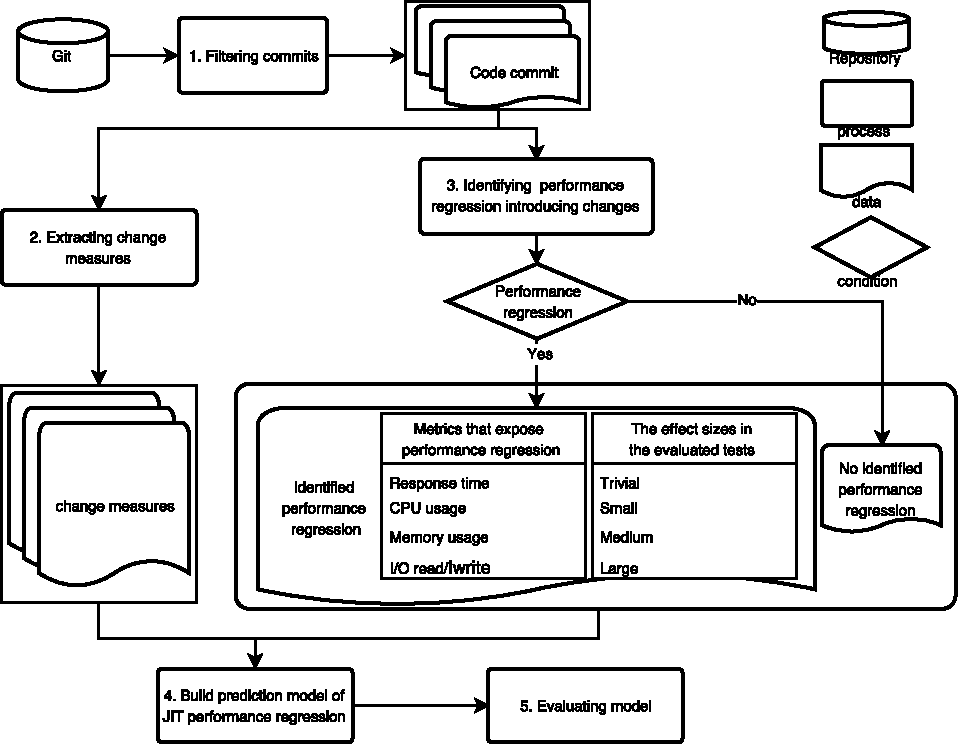
\includegraphics[width=\textwidth]{workflow}
	
	\caption{An overview of our approach that identifies performance regression introducing changes.}
	\label{fig:overview} 
\end{figure*}


\subsubsection{Filtering commits}
As the first step of our approach, we start off by filtering commits in order to focus on commits that are more likely to introduce performance regressions. In particular, we use \emph{git log} command to list all the files that are changed in each commit. We only extract the commits that have source code changes, i.e., changes to \emph{$.$java} files. 

%The purpose of filtering commits is to determine the versions and the analytic commits. In the first step, we determine the versions of \emph{Hadoop} and \emph{RxJava}. We clone the two open-source project by \emph{git log} command. Then we extract all the commits in limitation of two arbitrary releases or versions (\emph{Tag1} and \emph{Tag2})  by \emph{grep} tool.  Because the changes between each pair commits consists of  \emph{xml}, \emph{html}, \emph{txt}, \emph{md} and \emph{java} file changes. Finally, we filter the commits that contain java file change.


\subsubsection{Preparing impacted tests}

\noindent \textbf{Identifying impacted tests.} In order to evaluate performance of each code commit, we use the tests and performance micro-benchmarks that are readily available in the source code of our subject systems. As mature software projects, each subject system consist of a large amount of test cases. For example, \emph{Hadoop} release2.7.2 contains 1786 test cases in total. Exercising all test cases may cause two issues to our performance evaluation: 1) the test cases that are not impacted by the code change would dilute the performance impact from the code changes and introduce noise in the performance evaluation and 2) the large amounts of un-impacted test cases would requires extra resources for performance evaluation (e.g., much longer test running time). 

Therefore, in this step, we leverage a heuristic to identify impacted tests for each commit. In particular, we find that \emph{Hadoop} test cases follow a naming convention that the name of the test files contain that same name of the source code files being tested. For example, a test file named \emph{TestFSNamesystem.java} tests the functionality of \emph{FSNamesystem.java}. Hence, for each changed source code file in a commit, we automatically identify the test files. 

\noindent \textbf{Dealing with changed tests.} Some commits may change source code and test code at the same time. Such changed test cases would bias the performance evaluation if much testing logic is added, removed or modified in the test cases. In order to minimize the impact of changed test cases in performance evaluation, we opt to use the test code before the code change, since the new version of the test cases may include new features of the system, which is not the major concern of performance regression. However, in the cases where old test cases cannot compile or failed, we use the new test cases, since the failure of the compilation or the tests indicates that the old feature may be outdated. Finally, if both new and old test cases are failed or un-compliable, we do not include this test in the performance evaluation. In total, we have 132 tests with 106 commits that use the new tests to evaluate performance and 21 test with 19 commits that are not included in our performance evaluation. There exist only six commits that are not included at all because all of their tests are either un-compliable or failed.

\noindent \textbf{Leveraging micro-benchmarks for \emph{RxJava}. }Fortunately, \emph{RxJava} provides a slew of micro-benchmarks with the goal of easing performance evaluation. We find that these performance micro-benchmarks are designed to evaluate performance of the software as a cross-cutting concern, instead of evaluating any particular features separately. Therefore, we opt to run all 76 micro-benchmarks from \emph{RxJava}. In the rest of this paper, we also refer these micro-benchmarks as test cases to ease the description of our results.



%$The goal of this step is to parse the commit log and generate the regression tests or performance micro-benchmarks. The pseudocode of identify impacted tests in \emph{Hadoop} is shown in algorithm 1. The input contains the project name and two release tags and the output is the performance regression tests or performance micro-benchmarks.


	
%Based on pairwise commits analysis we compare every two consecutive commits (\emph{commit} is a current commit and \emph{pcommit} is its parent commit) and get the file changes. In \emph{Hadoop} \emph{java} changes contains source code changes and test code changes. In order to ensure the test cases can cover the source code changes and simultaneously exclude the performance effect of test code changes, we category two kinds of test cases. One is that there is no corresponding test code changes in the code changes. In this case, the test code is the same in \emph{commit} and \emph{pcommit} so run any test case is the same. Another is that the source code and the corresponding test code change together. This situation is more complex than the former case. In order to collect all the performance effect of the source code changes we run both test java cases on the current commit \emph{commit}. Also run both the test java cases on the parent commit \emph{pcommit}. We return all the test cases and the corresponding commits by \emph{array}. In \emph{RxJava}, we only consider the commits that contain java code changes. And we extract the performance micro-benchmarks directly. Finally, for the purpose of testing automatically and efficiently we transform and format our impacted tests and performance micro-benchmarks in a fixed style. Each row is triple. The first column represents the test commit, including current commit and its parent commit. The second column is the separator \emph{\#} so as to distinguish the commit and test case. The last column indicates the impacted test case or benchmarks test.


\subsubsection{Evaluating performance}

In this step, we exercise the prepared test cases and the performance micro-benchmarks to evaluate performance of each commit. We setup our performance evaluation environment based on Azure node type Standard F8s (8 cores, 16 GB memory). In order to generate statistically rigorous performance results, we adopt the practice of repetitive measurements~\cite{peterfse} to evaluate performance. In particular, each test or performance micro-benchmark are executed 30 times independently. We collect both domain level and physical level performance metrics during the tests. We measure the response time of each test case as domain level performance metric. A shorter response time indicating better performance of the software. We use a performance monitoring software named \emph{psutil}~\cite{psutil} to monitor physical level performance metrics, i.e., the CPU usage, Memory usage, I/O read and I/O write of the software, during the test.





%Evaluating performance will execute the test and gather the performance metrics. Performance regression testing aims to test the new program release more efficiently and locate the problematic bugs effectively. Regression testing is an iterative process because there are quite a lot of commits between two releases and there are numbers of test cases between two consecutive commits. In order to observe the performance effect of every single test case or micro-benchmark and prevent one test case influencing another test case, we run each test case individually rather all the test cases together. In the performance regression testing, we record the execution time by \emph{maven} tool in \emph{Hadoop} and \emph{gradle} tool in \emph{RxJava}. At the same time, we gather CPU, Memory and IO data by .

%To avoid outliers and be able to establish reliable statistical analysis we run each impacted test or micro-benchmark 30 times and collect the performance metrics. After gathering performance data together, we remove the outliers due to some totally different execution logs because of system exception or other reasons. On the other hand we rerun the impacted test or micro-benchmark again until the number of executions is 30. The Runtime, Memory, CPU and IO measured data is not uniform so data preprocess has to be applied to tackle this problem, including adopting unified stored format and the unit of measurement.

\subsubsection{Statistical analyses on performance evaluation}

Statistical tests have been used in prior research and in practice to detect whether performance metric values from two tests reveal performance regressions \cite{AlGhmadi}. After having the performance evolution results, we perform statistical analyses to determine the existence and the magnitude of performance regression in a statistically rigorous manner. We use Student’s t-test to examine if there exists statistically significant difference (i.e., p-value $<$ 0.05) between the means of the performance metrics. A p-value $<$ 0.05 means that the difference is likely not by chance. 
A t-test assumes that the population distribution is normally distributed. Our performance measures should be approximately normally distributed given the sample size is large enough according to the central limit theorem \cite{Chen:2014}.

T-test would only tells us if the differences of the mean between the performance metrics from two commits are statistically significant. On the other hand, effect sizes quantify such differences. Researchers have shown that reporting only the statistical significance may lead to erroneous results (i.e., if the sample size is very large, p-value can be small even if the difference is trivial). We use \emph{Cohen\textquotesingle s d} to quantify the effects~\cite{ES2006:Becker}. \emph{Cohen\textquotesingle s d} measures the effect size statistically and has been used in prior engineering studies~\cite{IST2007:Kampenes, ICSE2002:Kitchenham}. \emph{Cohen\textquotesingle s d} is defined as:
$$
Cohen\textquotesingle s \ d=\frac{mean(x1)-mean(x2)}{s}
$$
where \emph{mean(x1)} and \emph{mean(x2)} are the mean of two populations, and s is the pooled standard deviation~\cite{JohnWiley:2011}.
$$
\mathit{effect \ size} = \left\{ \begin{array}{ll}
trivial & \textrm{if $Cohen\textquotesingle s \ d  \leqslant 0.2$}\\
small & \textrm{if $0.2 < Cohen\textquotesingle s \ d \leqslant 0.5$}\\
medium& \textrm{if $0.5 < Cohen\textquotesingle s \ d \leqslant 0.8$}\\
large& \textrm{if $0.8 < Cohen\textquotesingle s \ d$}
\end{array} \right.
$$

\end{comment}
